\chapter{Implementation}\label{s:Implementation}

\graphicspath{ {./images/} }
    \begin{figure}
        \centering
        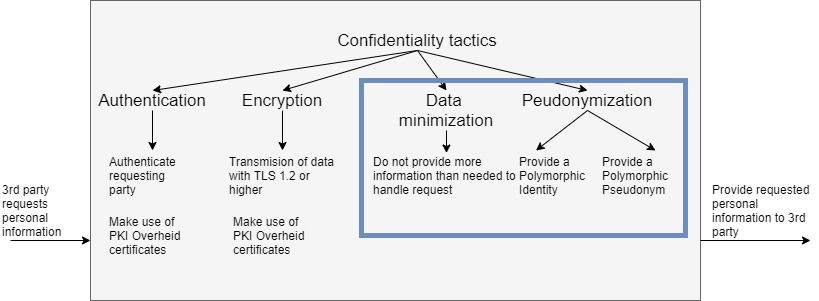
\includegraphics[width=14cm]{Tactics.jpg}\\
        \caption{Confidentiality tactics - next section handles examples in blue frame}
        \label{fig:Tactics}
    \end{figure}

Research question 3 focuses on patterns and tactics in context of software architecture which can be used to mitigate identity fraud. Bass \etal \cite{Bass2015SoftwareAI} mentions the following regarding architectural patterns "Compositions of architectural elements and provide packaged strategies for solving some of the problems facing a system." This section applies patterns and tactics based on examples of processes represented by views as referred to by Krutchen \cite{Krutchen1995ArchitecturalB}. Quality attribute 'Confidentiality' is identified as Quality attribute which could mitigate the operational problems of section \ref{OP}. Input of consulted experts have marked the methods of 'Zero-knowledge proof' and 'Data minimization' as examples of use-cases. 'Pseudonymization' is defined in GDPR Article 4(5) and Article 25 \cite{GDPR} and therefore deemed relevant to explicitly describe the definition and possible solution. Depicting different types of views of example processes embedding these methodologies, will make it more tangible for practical use. The tactics of 'Authentication' and 'Encryption' are argued to implement or otherwise explain why it has not been implemented by Dutch governmental architectural standards \cite{NORA_PasToeOfLegUit}. These standardized building blocks are important to have in place and explained briefly.


\section{Zero-knowledge proof}
By definition of Goldwasser \etal \cite{Goldwasser} "A zero-knowledge proof (ZKP) makes it possible to prove a statement is true while preserving confidentiality of secret information". 
Xiaohui Yang and Wenjie Li \cite{YANG2020102050} state "Zero-knowledge proof (ZKP) is a cryptography technique, which means that the prover can convince the verifier that a certain statement is correct without providing the verifier with any additional information or leaking any information about the witness." Figure \ref{fig:ZKP_usecase} presents a schema on how this principle works. Figure \ref{fig:QAS01} presents two example Quality Attribute Scenarios (QAS) which describe desired system behaviour of this example process. ZKProof Community reference \cite{2019:zkproof:community-reference-0.2} of Bennarroch \etal has been used as a source for creativity and is intended to provide a reference for development of zero-knowledge proof by contribution of world-renowned cryptographers, practitioners and industry leaders. Section \ref{OP} mentions the operational problems. If no identity data has to be shared or replicated, profiling or unauthorized correlation of identity data will not be possible. Not having identity data at all will also make it impossible to commit identity fraud. 
Zero-knowledge proof itself is a methodology which translates into a variety of possible technical implementations. This section contains an example of a high-level scenario and use-cases depicted in figure \ref{fig:ZKP_usecase}. However, suitability of this methodology needs to be assessed per use-case and possible other application besides this scenario. 

\subsection{Use-case description}\label{UC_description}
    
    \begin{figure}
    \graphicspath{ {./images/} }
        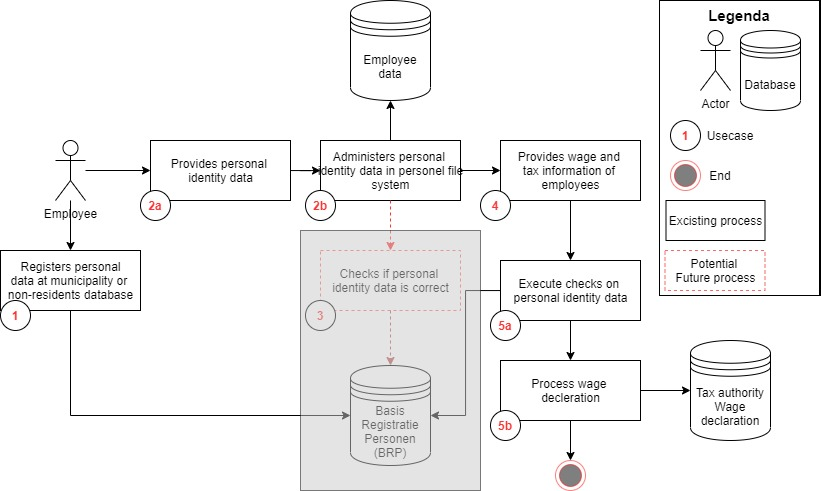
\includegraphics[width=10cm]{Usecase for zkp.jpg}\\
        \centering
        \caption{Scenarios - set of use-cases on one of ZKP could be applied}
        \label{fig:ZKP_usecase}
    \end{figure}


    \begin{figure}
        \graphicspath{ {./images/} }
        \centering
        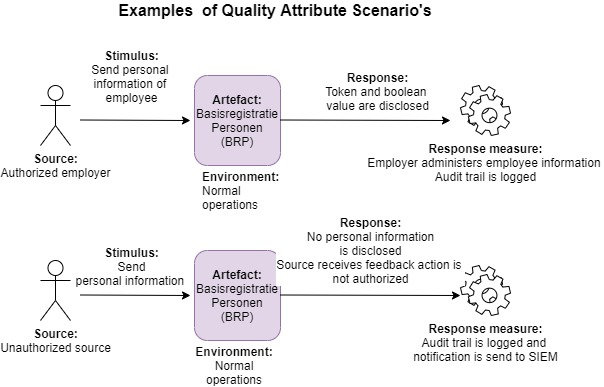
\includegraphics[width=7cm]{QAS-01 ZKP.jpg}\\
        \caption{Example of Quality attribute scenarios}
        \label{fig:QAS01}
    \end{figure}

This use-case contains three acting parties, namely the employee, the employer and the tax authorities (Belastingdienst).
A citizen finishes its registration of personal data at a municipality or non-residents database desk. After this process is finished the citizen receives a BSN, which serves as a UIN throughout all government administrations (phase 1). The citizen starts working at an employer, fills in his personal information for the wage declaration, including the BSN (phase 2a). The employer is responsible for administering personal information of its employees (phase 2b) and administering and transferring wage declarations to the tax authorities (phase 4). Based on the BSN in the wage declaration, the tax authority checks the personal identity data (phase 5a). \par
In the happy flow, all information of the employee is correct and the wage declaration is processed correctly (phase 5b). However, there are practical exceptions, where an employer administers an incorrect BSN or the set of personal information does not match that BSN. In this case, the wage declaration is processed incorrectly. Impact can be another citizen, with the wrongly entered BSN, being taxed for the wage of a different citizen. Correcting these mistakes are costly for the government and intense for a citizen who could be negatively impacted because of a higher wage and higher tax imposition.

\subsection{Use-case phase 3: Adding Zero-knowledge proof}
Letting an employer check the authenticity of personal information when hiring a citizen could solve the described problem. Section \ref{BRP} describes the BRP as the central database of personal identity data of citizens and could be considered as a source. However, consulting the BRP by an employer is not legally allowed and one could argue it's not desirable in the future because of the risk of employers not acting in good faith. This could result in individuals scraping the BRP database to commit fraud or unauthorized usage of personal data mentioned in section \ref{OP}. Zero-knowledge proof could be a method to resolve this problem by providing a check on personal information of an employee by the employer. The employer sends in information to a service (website or API/webservice) containing a set of personal information of the employee. The response will present a Boolean value True which will confirm that the personal information matches the BRP data or False indicating that the employee needs to provide the correct personal information to the employer. Of course, authentication of the employer is needed as is encryption of website or API/webservice. Desired behaviour is described in Figure \ref{fig:QAS01}.

This solution could be considered as an intermediate step in implementing a form of Zero-knowledge proof. Ultimately, having a validation token provided by trusted parties and no personal information at all in an employer database would be an end-state situation for Zero-Knowledge proof. However, law mandates an employer to have a personal file containing personal information of its employees. Discussions and required changes on law are out of scope for this research meaning only a solution within the scope of current law is provided.
\clearpage

\section{Data minimization} \label{data-minimization}

GDPR \cite{GDPR} defines 'Data minimization' as "adequate, relevant and limited to what is necessary in relation to the purposes for which they are processed (‘data minimisation’).". The purpose of usage of personal information in the BRP is established by law, making it transparent for demanding parties which personal information they can retrieve from the BRP. However, it is still desirable to minimize the amount of exposed information.

\subsection{Use-case description}
Demanding parties of personal information who are legally permitted to consult the BRP need to search for a person of interest residing on an address. In this case it can be assumed the personal information that needs to be shown is only of the person of interest. A query which is too broad could give back results of multiple persons. Which could be considered a breach of privacy of those people. As discussed in Section \ref{scope} a data breach could result in illegally obtaining personal information. Figure \ref{fig:Adhoc} illustrates a logical view on how a tactic of data minimization could be applied to mitigate this risk. A selection of possible addresses is queried on the Basisadministratie Gebouwen (BAG) \cite{BAG} which is a publicly accessible database (phase 1). The BAG contains almost all addresses within the Dutch territory. The correct address is selected from the query output (phase 2). If the query is a specific statement and returns one result, this result can be selected automatically to support usability. Based on the unique address ID from the BAG a list of residents is shown if the demanding party is authorised to consult the BRP (phase 3). A minimal set of personal information is shown to assess if the results contain the person of interest (phase 4). If the person of interest is identified as present in this list, the BRP is checked again for attributes which the demanding party can view (phase 5) and the personal information is retrieved and shown to the demanding party (phase 6).
    
    \begin{figure}
        \graphicspath{ {./images/} }
        \centering
        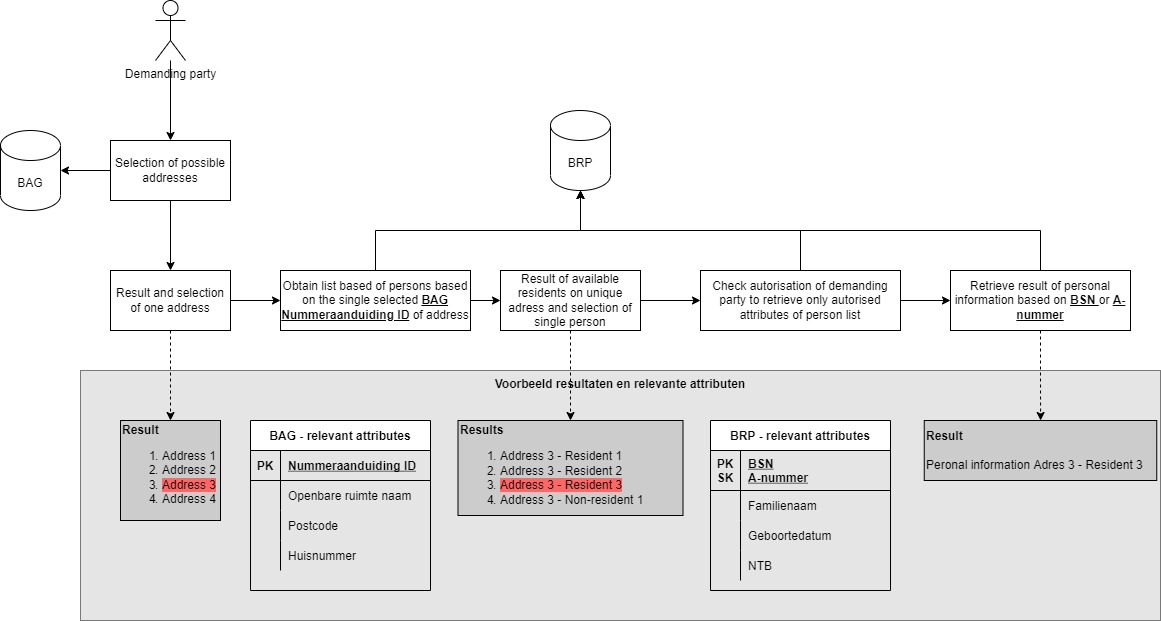
\includegraphics[width=14cm]{Ad-hoc adresvraag dataminimalisatie-EN.jpg}\\
        \caption{Logical view - example of data minimization in a process}
        \label{fig:Adhoc}
    \end{figure}

\section{Pseudonymization - Polymorphic Identity or Polymorphic Pseudonym}
GDPR \cite{GDPR} mentions the following regarding ‘pseudonymisation': "means the processing of personal data in such a manner that the personal data can no longer be attributed to a specific data subject without the use of additional information, provided that such additional information is kept separately and is subject to technical and organisational measures to ensure that the personal data are not attributed to an identified or identifiable natural person". The Digital Authentication Guideline of National Institute of Standards and Technology (NIST) provides requirements to identity providers called pairwise Pseudonymous identifiers \cite{NIST_800-63C}. If a unique identifier of a person needs to be shared while this identifier itself is not relevant for the demanding party, it does not need to be revealed to that party and can be provided as a pseudonym. Requirements within the NIST guideline prescribe tracing that unique person with other attributes should not be possible. Therefore, not scoping pseudonymization not only to a UIN.

This technique has been already applied in a governmental service BSNk \cite{Logius_BSNk} and describes in work by Erik Verheul \cite{VerheuleID}.

\section{Supporting tactics}

\subsection{Authentication} \label{authentication}
Definition: "Authentication is the process of recognizing a user’s identity. It is the mechanism of associating an incoming request with a set of identifying credentials. The credentials provided are compared to those on a file in a database of the authorized user’s information on a local operating system or within an authentication server." \cite{authentication}
A commonly used method for authentication purposes is usage of a certificate. Parties who communicate with or on behalf of the Dutch government are issued a PKIoverheid (PKIO) certificate. These certificates are implemented in machine to machine interfaces like APIs and used for authentication, electronic signatures and encryption. \cite{Logius_PKIO}

\subsection{Encryption - Transfer of data is encrypted with TLS 1.2 or higher} \label{encryption}
Encryption of data in transfer is used to prevent unauthorized access and data breaches. A broadly implemented standard is TLS. The Dutch reference architecture NORA (Nederlandse Overheid Referentie Architecture) \cite{NORA} states this standard needs to be applied or otherwise explained why it has not been implemented \cite{NORA_PasToeOfLegUit}. On the part of TLS it is clear version 1.2 or higher is accepted, but version 1.3 is preferred \cite{NORA_TLS}. 

\section{Confirmation, gaps and trade-offs}
Suggested solutions and argumentation is based on the Quality attribute of Confidentiality which is deemed an Architecturally Significant Requirements. Besides Confidentiality there are four other Architecturally Significant Requirements. Possible gaps and trade-offs of these solutions are composed by logical reasoning and discussed in Table \ref{tab:Trade-offs} and expanded before implementation.

\subsection{Definition of residual ASRs}
Prior to the assessment of the suggested solutions on other Quality attributes a definition is required of the other QA's. ISO 25010 \cite{ISO:25010:2011} defines these Quality attributes: \\
\textit{Reusability (part of Maintainability)} - Degree to which an asset can be used in more than one system, or in building other assets. \\
\textit{Maturity (part of Reliability)} - Degree to which a system, product or component meets needs for reliability under normal operation. \\
\textit{Authenticity (part of Security)} - Degree to which the identity of a subject or resource can be proved to be the one claimed. \\
\textit{Accountability (part of Security)} - Degree to which the actions of an entity can be traced uniquely to the entity. \\

\begin{longtable}[c]{|p{3cm}|p{3cm}|p{3cm}|p{3cm}|p{3cm}|p{3cm}|}
 \caption{Solutions and conformity to other ASRs\label{tab:Trade-offs}}\\
 \hline
 \multicolumn{6}{| c |}{Begin of Table}\\
 \hline
& Reusability & Maturity & Authenticity & Accountability \\
 \hline
 \endfirsthead

 \hline
 \multicolumn{6}{| c |}{Continuation of Table \ref{tab:Trade-offs}}\\
 \hline
   & Reusability & Maturity & Authenticity & Accountability \\
 \hline
 \endhead

 \hline
 \endfoot

 \hline
 \multicolumn{6}{| c |}{End of Table}\\
 \hline\hline
 \endlastfoot
  Zero-Knowledge proof & ZKP is a base for Blockchain applications. However, it can be applied more broadly and even without usage of the blockchain. & Depending if it will be in a blockchain or independent instances of servers. It can be argued the broad applications of blockchain, beside crypto currencies, are scarce &  It can be argued privacy preserving solutions are in less need of this QA, having no information leaked when a breach occurs. However, it's needed to assume illegal actions can always occur and need to be mitigated by at least authenticating parties. & It can be argued privacy preserving solutions are in less need of this QA, having no information leaked when a breach occurs. However, logging and monitoring should be defined as a requirement. \\
 \hline
  Data-minimization & The method itself can be argued as reusable. However, it can be possible to have adapted applications per type of usage of personal information. Resulting in customization and possible various methods of data-minimization. & From a technological stand the technique can be applied widely. Bounded rationale \cite{simon} by software architects could lead to not implementing because of current patterns of delivering data work. & Establishing prove of the identity of a demanding party is needed to preserve the privacy even if the provided data is minimized. & Personal information is provided, implicating the provider is obligated by law \cite{GDPR} on providing an audit trail. \\
 \hline
  Pseudonymization & Providing the method as a service like BSNk \cite{Logius_BSNk} will facilitate adoption and possible future applications & Pseudonymization can be implemented through different types of algorithms. Therefore, it's needed to select the appropriate algorithm that fits the desired reliability.  & Besides pseudonymization GDPR \cite{GDPR} Article 32 prescribes "the ability to ensure the ongoing confidentiality, integrity, availability and resilience of processing systems and services". Thus, needing to authenticate demanding parties of personal information & Personal information is provided, implicating the provider is obligated by law \cite{GDPR} on providing an audit trail. \\
 \hline
  Authentication with PKIO certificates & Authentication by means of certificates is broadly reused and therefore deemed to conform with this QA & Authentication by means of certificates is a broad standard and therefore deemed to conform with this QA & Authentication is defined as the process to prove Authenticity and therefore deemed to conform with this QA & Personal information is provided. implicating the provider is obligated by law \cite{GDPR} on providing an audit trail.\\
 \hline
 Encryption with TLS 1.2 or higher & Encryption with TLS is a broad standard and therefore deemed to conform with this QA & Encryption with TLS is a broad standard and therefore deemed to conform with this QA & Encryption with TLS supports authenticity but needs additional technologies (for example certificate authentication).  & Encryption itself will not facilitate in this QA \\
 \hline
\end{longtable}

%%% Local Variables:
%%% mode: latex
%%% TeX-master: "../thesis"
%%% End: